\documentclass[12pt,a4paper]{article}

\usepackage{a4wide}
\usepackage{minted}
\usepackage{csvsimple}
\usepackage{amsmath}
\usepackage{booktabs}
\usepackage{amssymb}
\usepackage{nicefrac}
\usepackage{enumitem}
\usepackage{float}
\usepackage{todonotes}
\usepackage[breaklinks,plainpages=false,pdfpagelabels]{hyperref}
\hypersetup{colorlinks,citecolor=blue,filecolor=blue,linkcolor=blue,urlcolor=blue}
\usepackage{graphicx}
\setlength\parindent{0pt} % no paragraph indents
\setlength\parskip{6pt} % paragraph vertical spacing
\usepackage{circuitikz} % for circuit diagrams
\usepackage{pgfplots}
\usepackage{tikz}
\usetikzlibrary{positioning,shapes,shadows,arrows,calc}
\DeclareMathOperator{\sinc}{sinc} %sinc
\usepackage[normalem]{ulem} %strike out text using \sout

\usepackage{fancyhdr}
\pagestyle{fancy}
\fancyhead[L]{CSSE4010: Digital Doo-Hickeys}
\fancyhead[R]{Sem 2, 2023}


%---------------------------------------------------------------%
%                                                               %
%               environment definitions                         %
%                                                               %
%---------------------------------------------------------------%
\newcounter{boldalphcounter}
\renewcommand{\theboldalphcounter}{(\alph{boldalphcounter})}
\newenvironment{boldalphlist}{\begin{list}{\textbf{\theboldalphcounter}}%
  {\usecounter{boldalphcounter}}}{\end{list}}

\newcounter{alphcounter}
\renewcommand{\thealphcounter}{(\alph{alphcounter})}
\newenvironment{alphlist}{\begin{list}{\thealphcounter}%
  {\usecounter{alphcounter}}}{\end{list}}

\newcounter{romancounter}
\renewcommand{\theromancounter}{\roman{romancounter})}
\newenvironment{romanlist}{\begin{list}{\textbf{\theromancounter}}%
  {\usecounter{romancounter}}}{\end{list}}

\newcounter{boldarabiccounter}
\renewcommand{\theboldarabiccounter}{\arabic{boldarabiccounter}}
\newenvironment{boldarabiclist}{\begin{list}{\textbf{\theboldarabiccounter.}}%
  {\usecounter{boldarabiccounter}}}{\end{list}}

 % Counter
\newcounter{questioncounter}

\begin{document}

\begin{center}
\bigskip
\section*{CSSE4010 A3}
\end{center}

David Gaul

s4671313

Lab Session: Wednesday 10-12

Submission Date: 5th-ish September

\section{Introduction}

There were two separate tasks that were to be fulfilled for prac 3. These tasks were:

\begin{itemize}
    \item To create a 16-bit two's comp adder. This adder has to take two 16-digit inputs, as well as a carry-in. Depending on whether saturation was enabled or not, the output would either wrap around or set the two's comp ZNCV flags.
    \item To create a two-digit BCD adder. This process had to be complete by first creating a 1-digit BCD adder, before cascading it into the second.
\end{itemize}

Ready for another fun filled report???

LET'S GOOOOOOOO


\section{Block Diagram}

When discussing the project architecture, it's important to talk about the basics. To begin, this is an 8-bit register:

\begin{figure}[H]
    \centering
    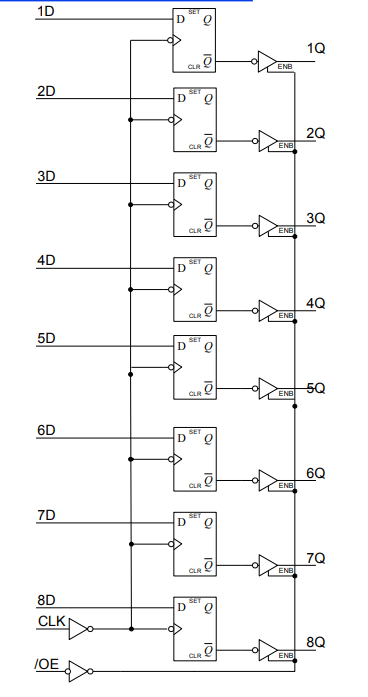
\includegraphics[scale=0.25]{images/register.png}
    \caption{Pictorial depiction of an 8-bit register}
    \label{fig:register}
\end{figure}

And this is the complete prac 3A architecture:

\begin{figure}[H]
    \centering
    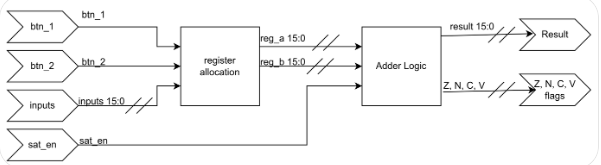
\includegraphics[scale=0.5]{images/block_diagram_a.png}
    \caption{Completed block diagram for part A}
    \label{fig:block_a}
\end{figure}

Confused? So am I.

The entire design was implemented in such a way that it could be tested on the Nexys 4 boards (And it eventually was, successfully, but the full integration is outside the scope of this assignment, and details are not included). The register allocation system received a 16 bit input line, as well as two buttons. Depending on which of these buttons was pressed, the 16-bit input buffer was saved into either register A or B. These registers are then added together within the adder logic, which returns the result of the addition along with any flag values. The rules of the flag values are as follows:

If saturation is enabled:
\begin{itemize}
    \item If a positive overflow occurs, 0x7FFF is returned, and the overflow flag is set high
    \item If a negative overflow occurs, 0x8000 is returned. The overflow flag is once again set high
    \item If the result is negative, the negative flag is set high
    \item If there is a carry out bit, the carry flag is set high
    \item If the result is 0, the zero flag is set high
\end{itemize}

If saturation is not enabled:
\begin{itemize}
    \item The carry out flag will be set high when there is a carry out bit
\end{itemize}

The architecture of part 3B was slightly more involved. It required the use of clock dividers, two cascaded BCD adders and a finite state machine which finally led into the seven-seg decoder. The fully architecture of this can be found within figure \ref{fig:block_b}

\begin{figure}[H]
    \centering
    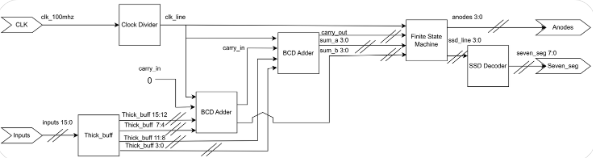
\includegraphics[scale=0.75]{images/block_diagram_b.png}
    \caption{Completed block diagram for part B}
    \label{fig:block_b}
\end{figure}

The clock divider has been included to help with synchronicity of the design. This was integral for use in the BCD adders, as well as the finite state machine, which controlled the outputs of the seven-seg display. 

Two cascaded BCD adders have been included. The input into each of the registers of the BCD adders is capped at nine. That is to say, each of the registers for the BCD adder have the following logic:

\begin{minted}{Python}
if input > 9:
    output <= 0;
else:
    output <= input;
\end{minted}

And the logic for a single BCD adder is:

\begin{minted}{Python}
if (carry_in = '1') then
    if (a_line + b_line + 1 < 10) then
        sum <= a_line + b_line + 1;
        carry_out <= '0';
    else
        sum <= a_line + b_line - 9;
        carry_out <= '1';
    end if;
else 
    if (a_line + b_line < 10) then
        sum <= a_line + b_line;
        carry_out <= '0';
    else
        sum <= a_line + b_line - 10;
        carry_out <= '1';
    end if;
end if;
\end{minted}

Essentially meaning that the output of the BCD adder will be the sum of the input registers plus the carry-in bit. If an overflow occurs, the carry-out bit will be set high and the result will be wrapped around by 10 (Which will display the correct output on the seven seg. This is essentially the equivalent of adding 6 to the design, as is recommended within the task sheet).

The carry-in to the first BCD adder is set to 0, as it is not required. The carry-out for the first adder connects to the carry-in for the second adder. In creating the adders in this fashion, it was possible to cascade the same design multiple times.

Finally, the finite state machine was used to output the result of the BCD addition onto the seven-seg display. Alternating on every rising clock edge, the FSM would output one of the three digits of the result onto the seven-seg display. The logic for this is as follows:

\begin{minted}{Python}
if rising_edge(clk_line) then

    if (alternator = 0) then
        anodes <= "11111011";
        if (carry_line = '1') then
            ssd_line <= "0001";
        else 
            ssd_line <= "0000";
        end if;
        alternator <= alternator + 1;
    elsif (alternator = 1) then
        anodes <= "11111101";
        ssd_line <= output_line(7 downto 4);
        alternator <= alternator + 1;
    else
        anodes <= "11111110";
        ssd_line <= output_line(3 downto 0);
        alternator <= 0;
        
    end if;
    
end if;
\end{minted}

Cool clarkies. Hope that makes sense.

\section{Simulation Results}

Once again, simulation results are kept intentionally brief. In this instance, there are $2^{17}$ possible combinations, which is far too many to write about in this document. For this reason, only key results have been included within the simulation. Full functionality can be verified during testing time.

For task 3A, the following tests were covered:

\begin{itemize}
    \item Initialising the simulated inputs to zero
    \item Inputting values of 1 and 0 (Which results in an output of 1, and verifies that summing is working)
    \item Inputting values of 1 and 8 (Which results in an output of 9 and further verifies summing functionality)
    \item Inputting two values of 0x7FFF to trigger a positive overflow (Overflow flag should trigger)
    \item Inputting two values of 0x8001 to trigger a negative overflow (Overflow, negative and carry-out flags should trigger)
    \item Inputting values of 0xFFFF and 0, to result in -1 and trigger the negative flag
    \item Inputting values of 0xFFFF and 0x0001 to result in 0. This will also trigger the carry-out flag
\end{itemize}

These tests were carried out both with saturation enabled, as seen in figure \ref{fig:sim_3a_sat_en}, and without saturation enabled \ref{fig:sim_3a_no_sat}.

\begin{figure}[H]
    \centering
    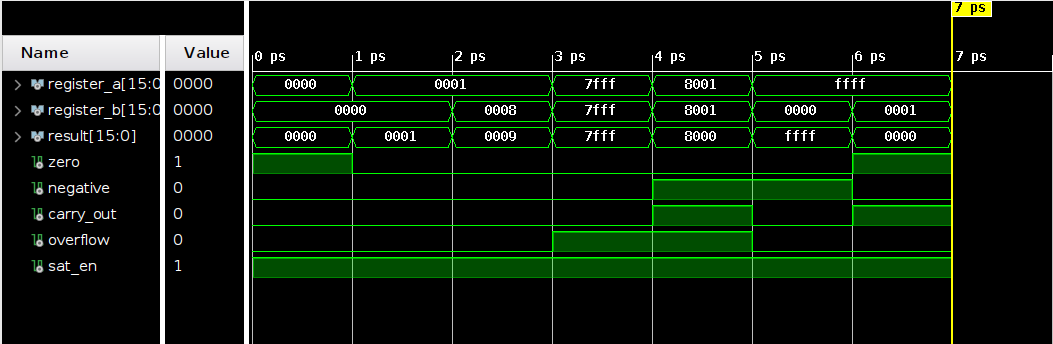
\includegraphics[scale=0.25]{images/sim_3a_sat_en.png}
    \caption{Simulation for part 3A with saturation enabled}
    \label{fig:sim_3a_sat_en}
\end{figure}

As can be seen within figure \ref{fig:sim_3a_sat_en}, the test cases were able to be input and resolved correctly by the system.

\begin{figure}[H]
    \centering
    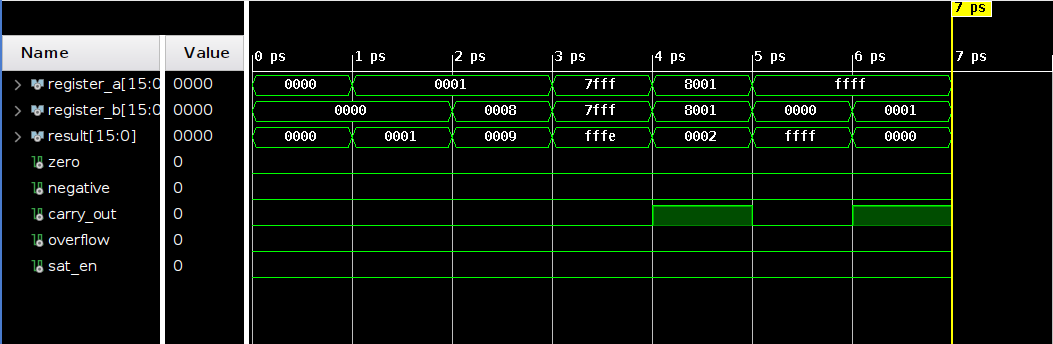
\includegraphics[scale=0.25]{images/sim_3a_no_sat.png}
    \caption{Simulation for part 3A with saturation disabled}
    \label{fig:sim_3a_no_sat}
\end{figure}

As can be seen in figure \ref{fig:sim_3a_no_sat}, the product works exactly as it did in the first case, except zero, overflow and negative flags were disabled. Only the carry-out flag was enabled. Another note-worthy feature of this test case is that the system wraps around when overflow occurs. In test cases where saturation was implemented, the addition of two 0x7FFF numbers triggered saturation. Without saturation, however, the result was 0xFFFE, indicating that wrap-around took place and the result became negative. This was further reflected with negative wrap-around resulting in 0x0002.

In total, the system is able to receive inputs, and will output the correct results, depending upon whether the saturation pin has been triggered. But the important part is that full functionality has been achieved.

For part 3B, more testing was required. At first, it was necessary to test the functionality of a single BCD adder, to confirm that it functioned as expected. From here, both BCD adders were placed in cascade fashion, and its functionality was once again verified.

\begin{figure}[H]
    \centering
    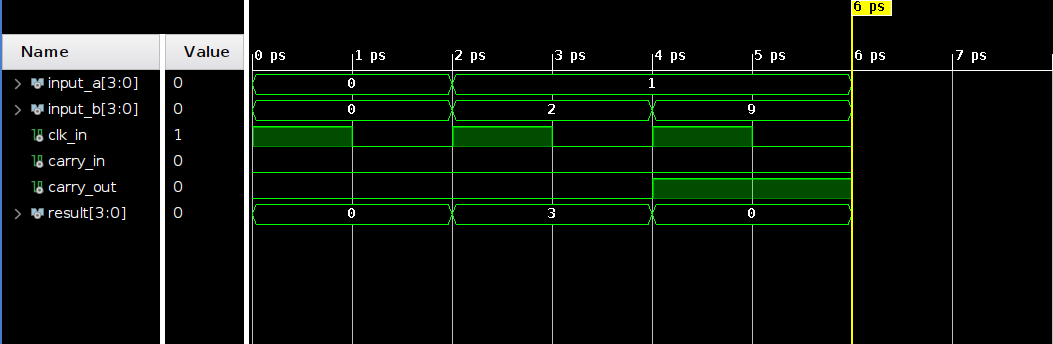
\includegraphics[scale=0.25]{images/sim_single_no_carry.png}
    \caption{Simulation for a single BCD adder with no carry-in}
    \label{fig:sim_single_no_carry}
\end{figure}

Figure \ref{fig:sim_single_no_carry} shows the following test cases, with no carry-in enabled:

\begin{itemize}
    \item Setting the inputs to 0, which results in an output of 0
    \item Setting the inputs to 1 and 2, which results in an output of 3
    \item Setting the inputs to 1 and 9, which triggers an overflow, setting the output to 0 and the carry-out bit to high
\end{itemize}

And as can be seen, the single adder performs as is expected. It's worth noting that neither of the inputs would exceed 9 during simulation. That is because a BCD adder does not take inputs of greater than 9. This test process was repeated with the carry-in bit enabled.

\begin{figure}[H]
    \centering
    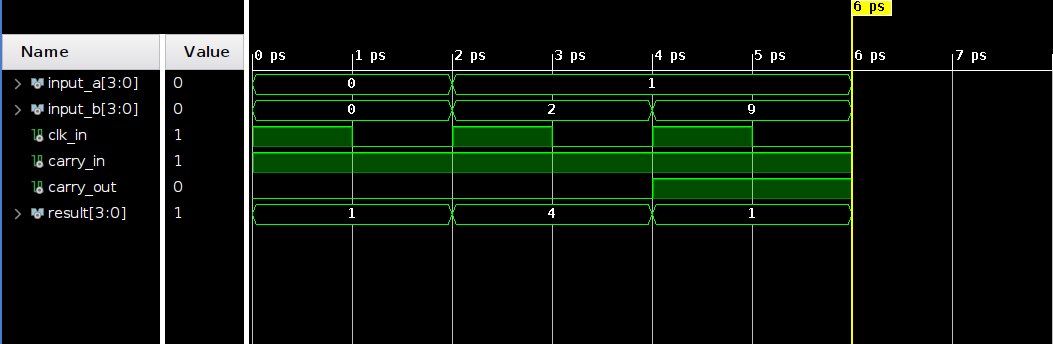
\includegraphics[scale=0.25]{images/sim_single_carry.png}
    \caption{Simulation for a single BCD adder with carry-in enabled}
    \label{fig:sim_single_carry}
\end{figure}

As can be seen in figure \ref{fig:sim_single_carry}, the outputs are identical to those in figure \ref{fig:sim_single_no_carry}, save that they've been increased by 1 to fascilitate the carry-in bit.

So in total the single adder works perfectly. From here, two single-bit BCD adders were cascaded together to form the two-digit BCD adder. The simulation for this featured the following test cases:

\begin{itemize}
    \item Inputting values of 0 into all inputs, which resets the ouptut to 0
    \item Inputting values of 2 and 1 into the lower bits, which results in an output of 0x03
    \item Inputting values of 9 and 1 into the lower bits. This triggers an overflow, and results in an ouput of 0x10
    \item Reseting the output to 0 by inputing 0x0000
    \item Inputting values of 2 and 1 into the higher bits, which results in an output of 0x30
    \item Inputting values of 9 and 1 into the lower bits. This triggers an overflow, and results in an ouput of 0x00, with the carry-out bit enabled
\end{itemize}

These test cases can be verified against the simulation shown in figure \ref{fig:sim_dual}.

\begin{figure}[H]
    \centering
    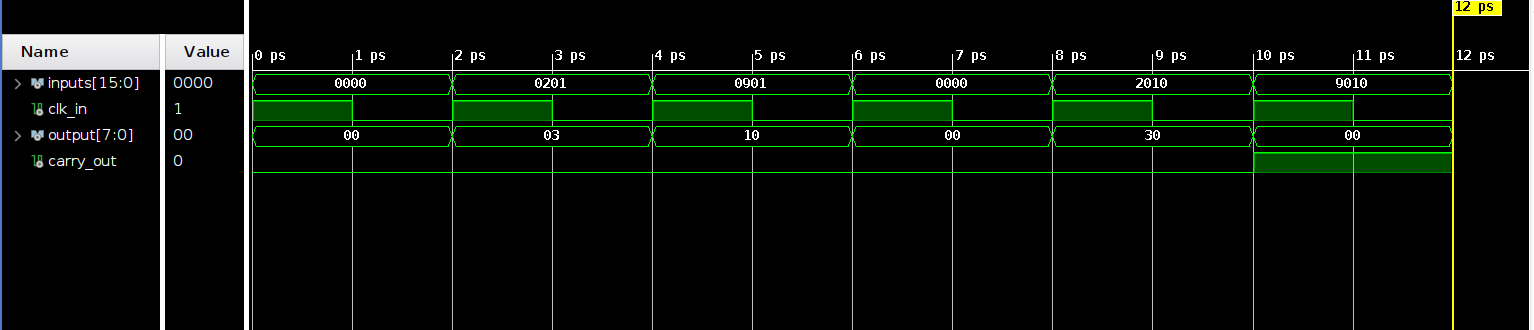
\includegraphics[scale=0.25]{images/sim_dual_adder.png}
    \caption{Simulation for the cascaded two-digit BCD}
    \label{fig:sim_dual}
\end{figure}

\section{Results on the FPGA}

To further verify the functionality of the design, it was uploaded onto the Nexys 4 FPGA. Several images were taken of the board operating as desired. Figure \ref{fig:fpga_base} shows the fpga with all switches disabled. Note that the output shown in this image is at 0x02. This is due to a broken pin on the board, not a design fault. Further information can be found on the Ed Discussion board about my broken FPGA.

\begin{figure}[H]
    \centering
    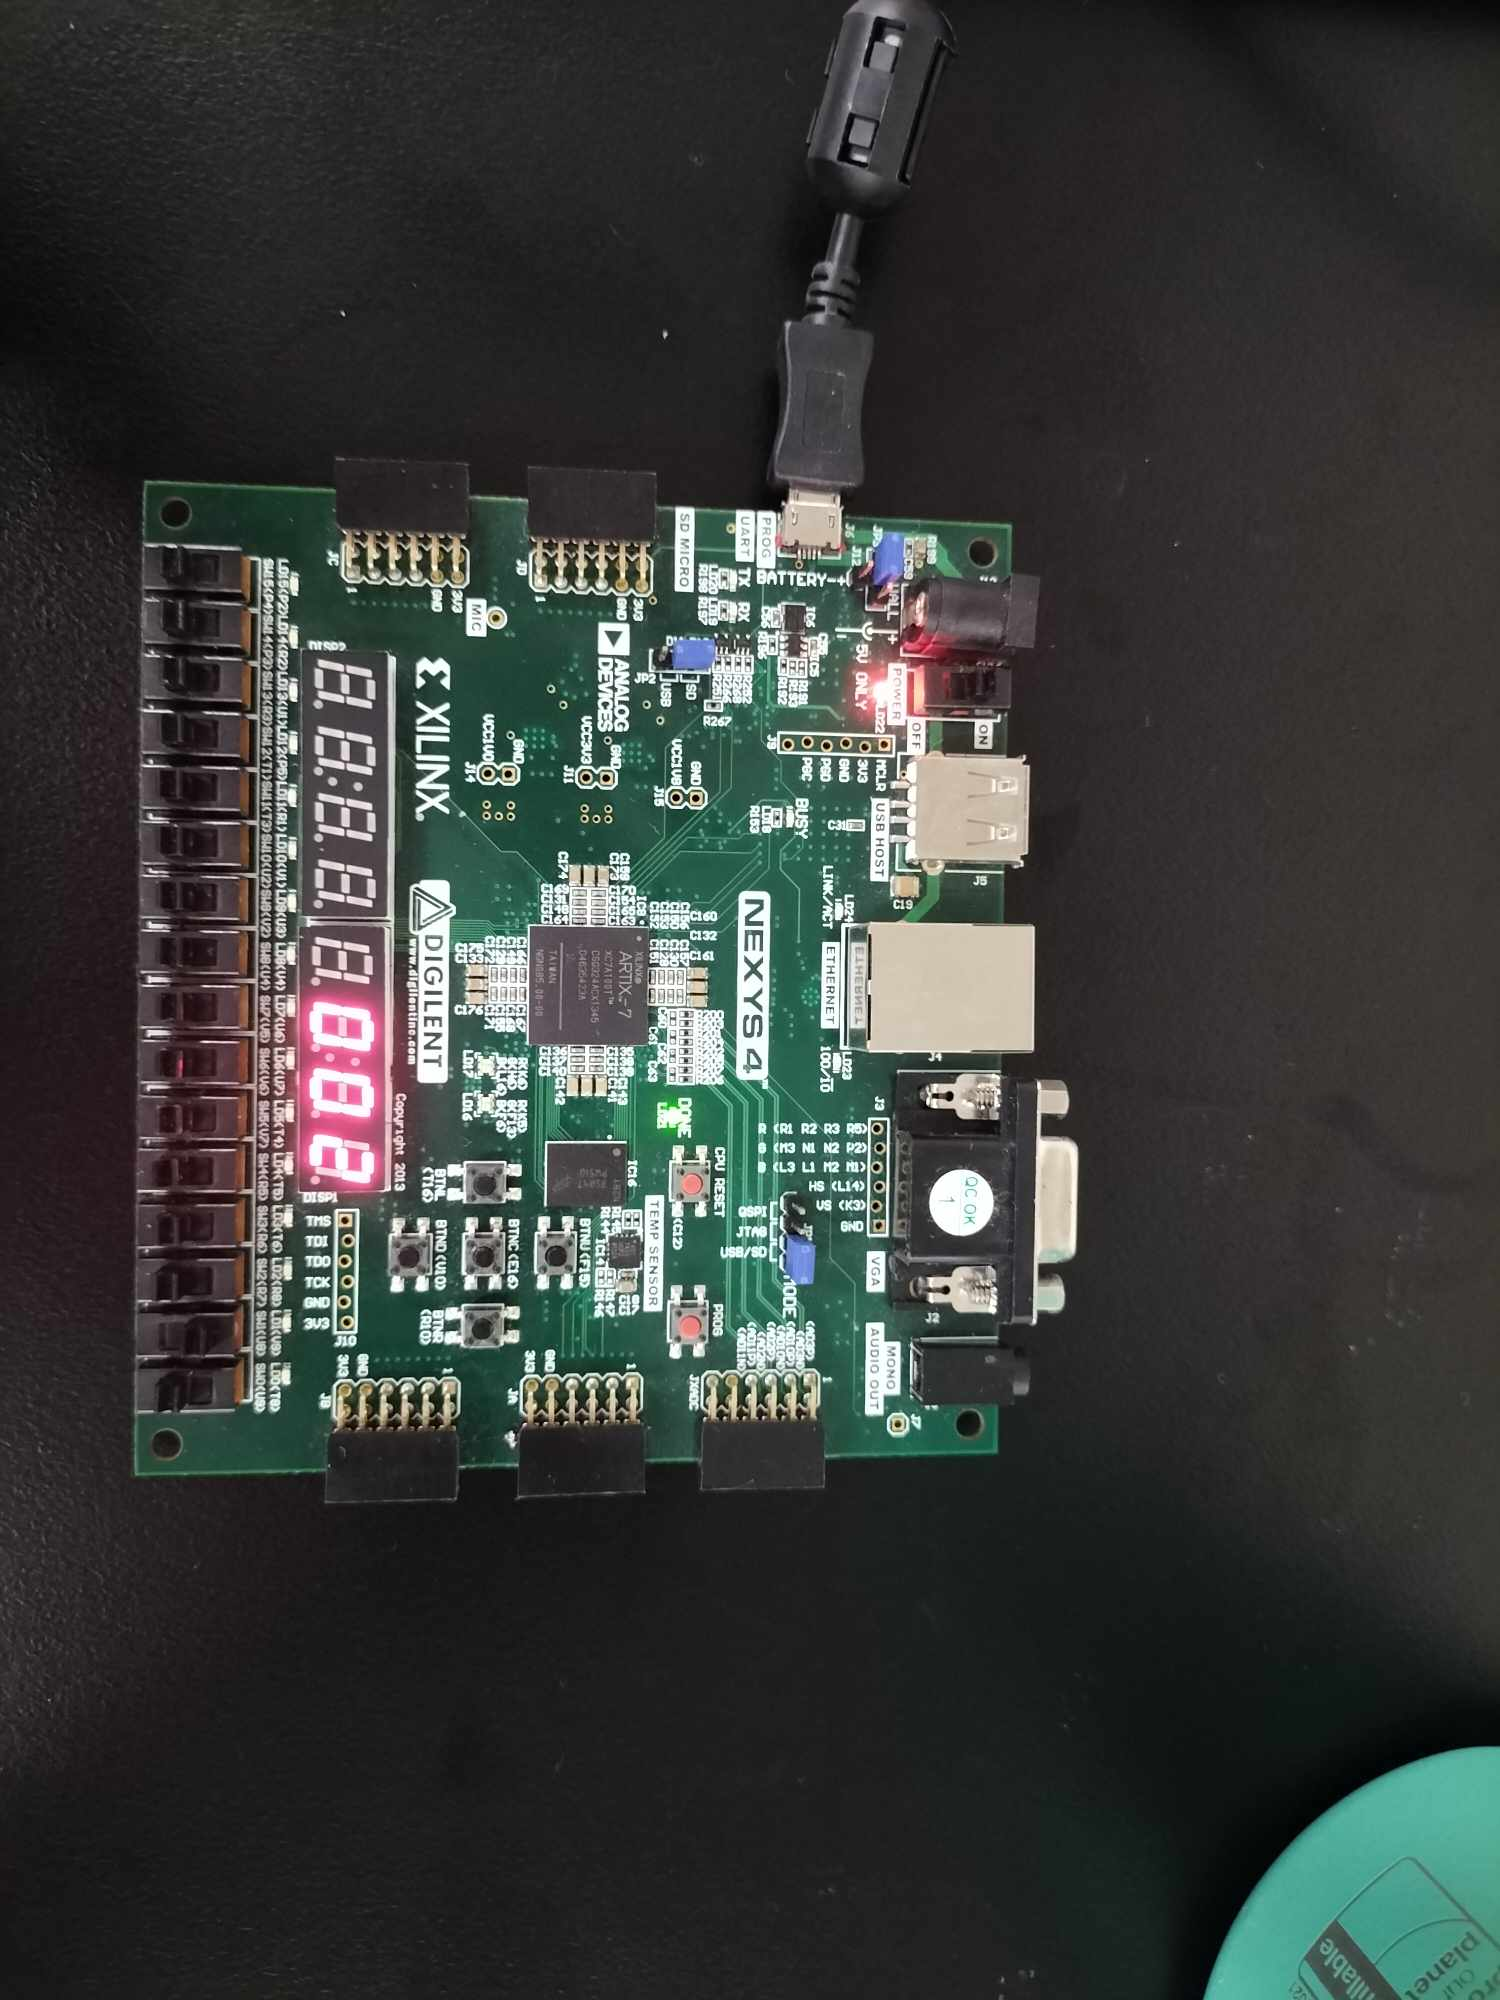
\includegraphics[scale=0.25]{images/fpga_base.jpg}
    \caption{Base state for FPGA with no switches enabled. Note that an output of 2 is present due to a broken pin. This has been talked about on the Ed Discussion board}
    \label{fig:fpga_base}
\end{figure}

Secondly, by inputing values of 0x92 and 0x12, the board returned a result of 0x104, which is exactly as expected. This helped to verify the overflow functionality.

\begin{figure}[H]
    \centering
    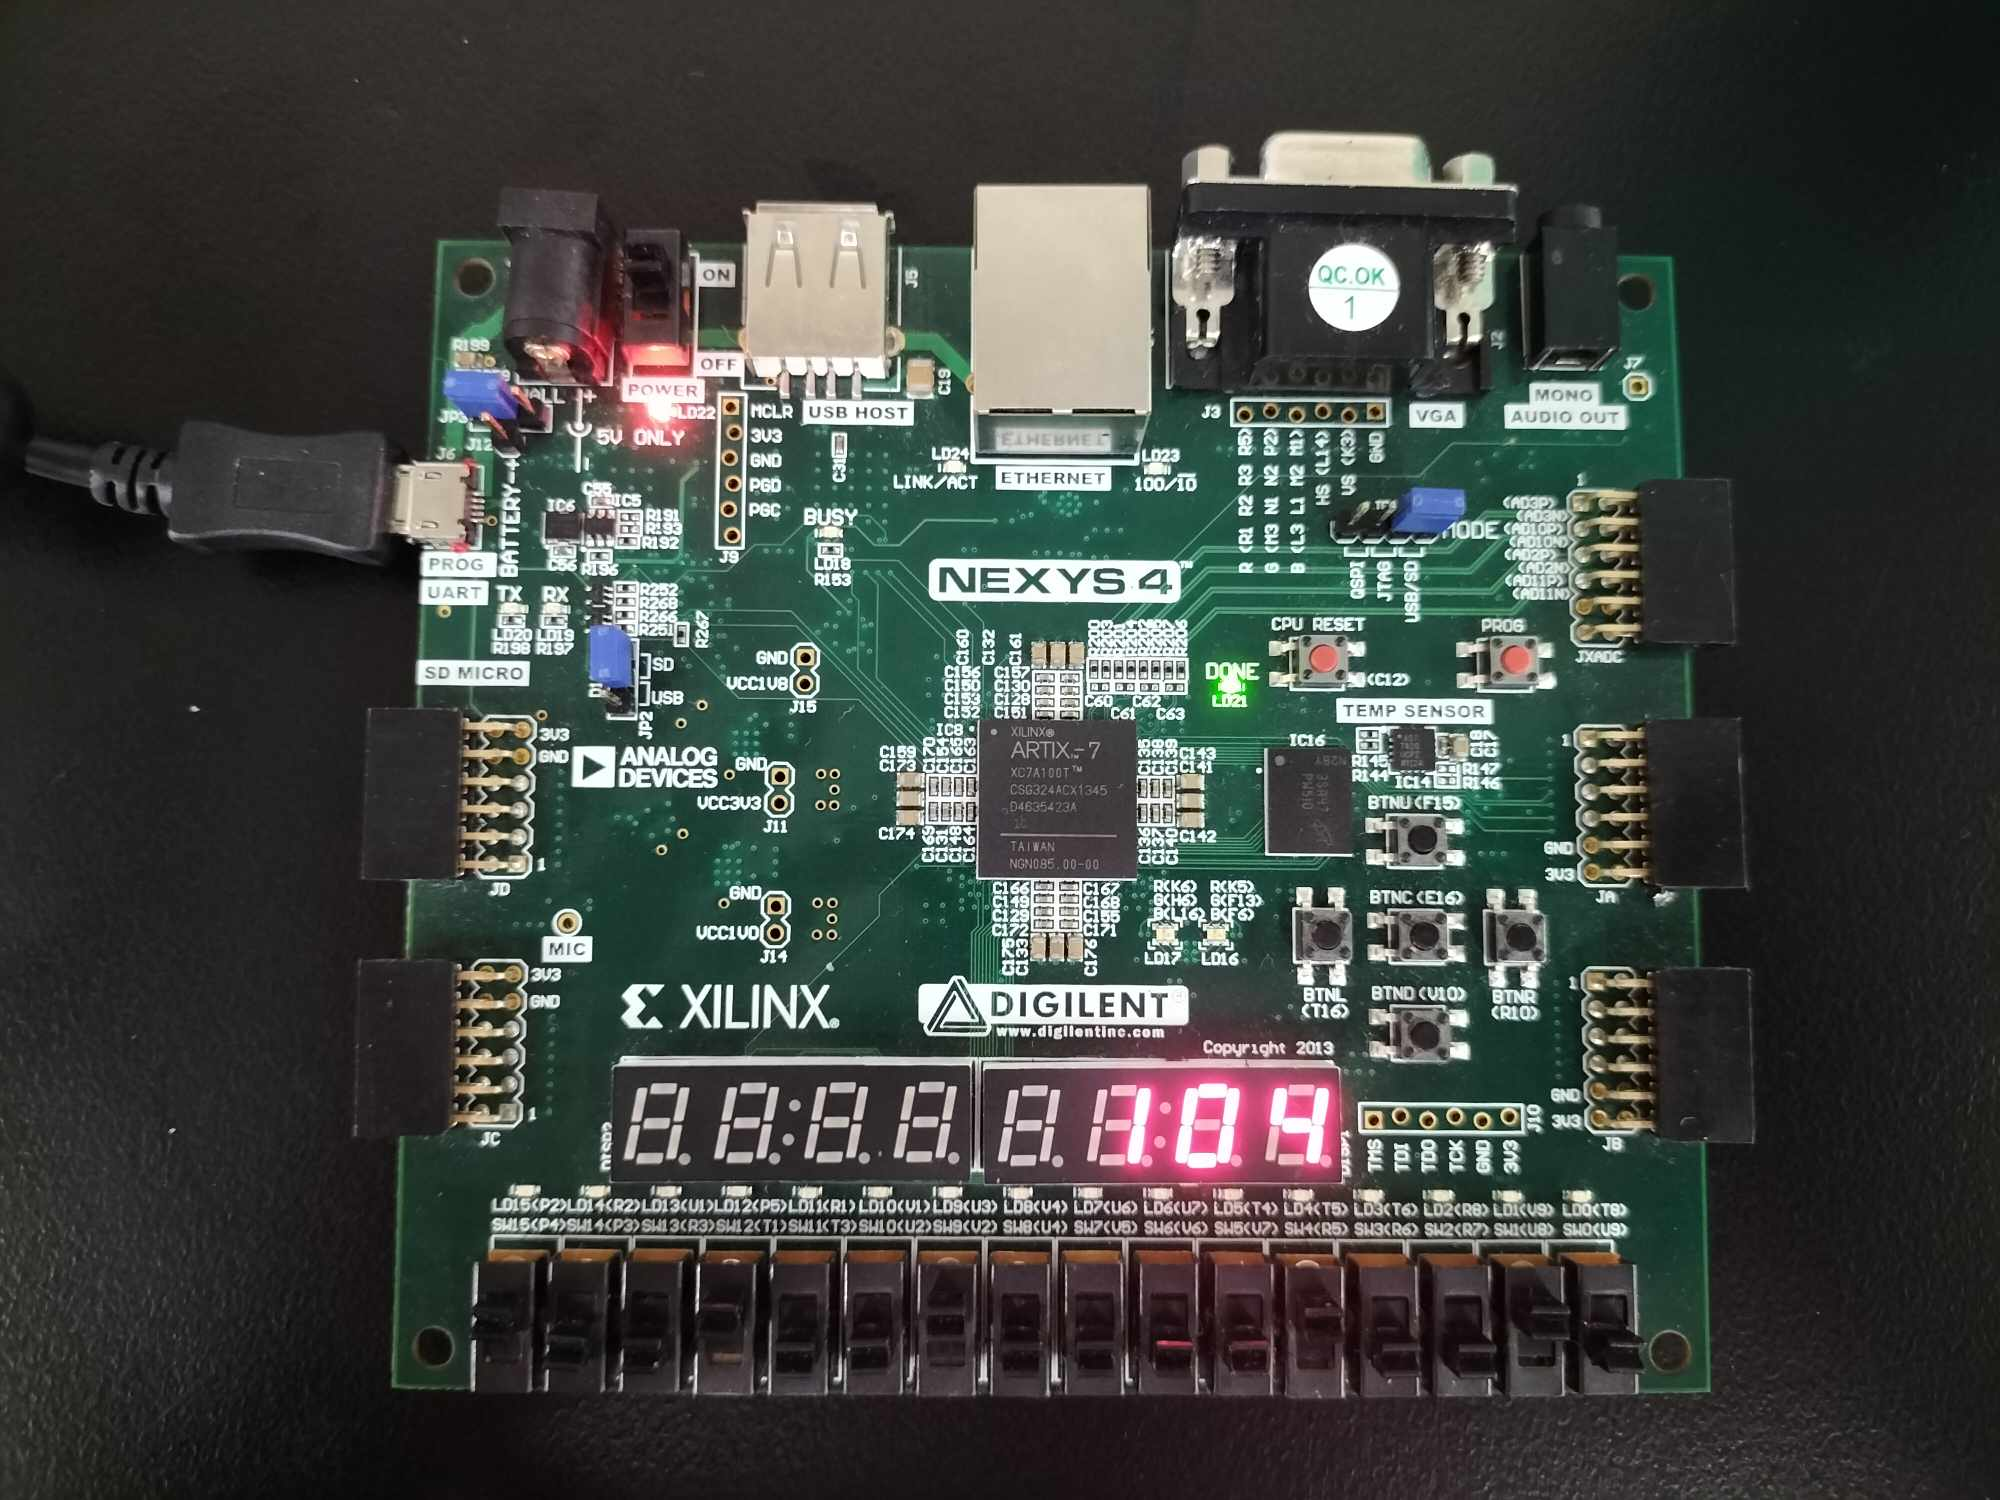
\includegraphics[scale=0.1]{images/fpga_1_overflow.jpg}
    \caption{FPGA with an overflow on the higher digit, and a total of 4 on the lower}
    \label{fig:fpga_one}
\end{figure}

Figure \ref{fig:fpga_two} shows the final test case on the board, where 0x96 and 0x16 were input into the board, resulting in 0x112.

By this point, it can be safely verified that all major test cases have been satisfied and the board functions as expected.

\begin{figure}[H]
    \centering
    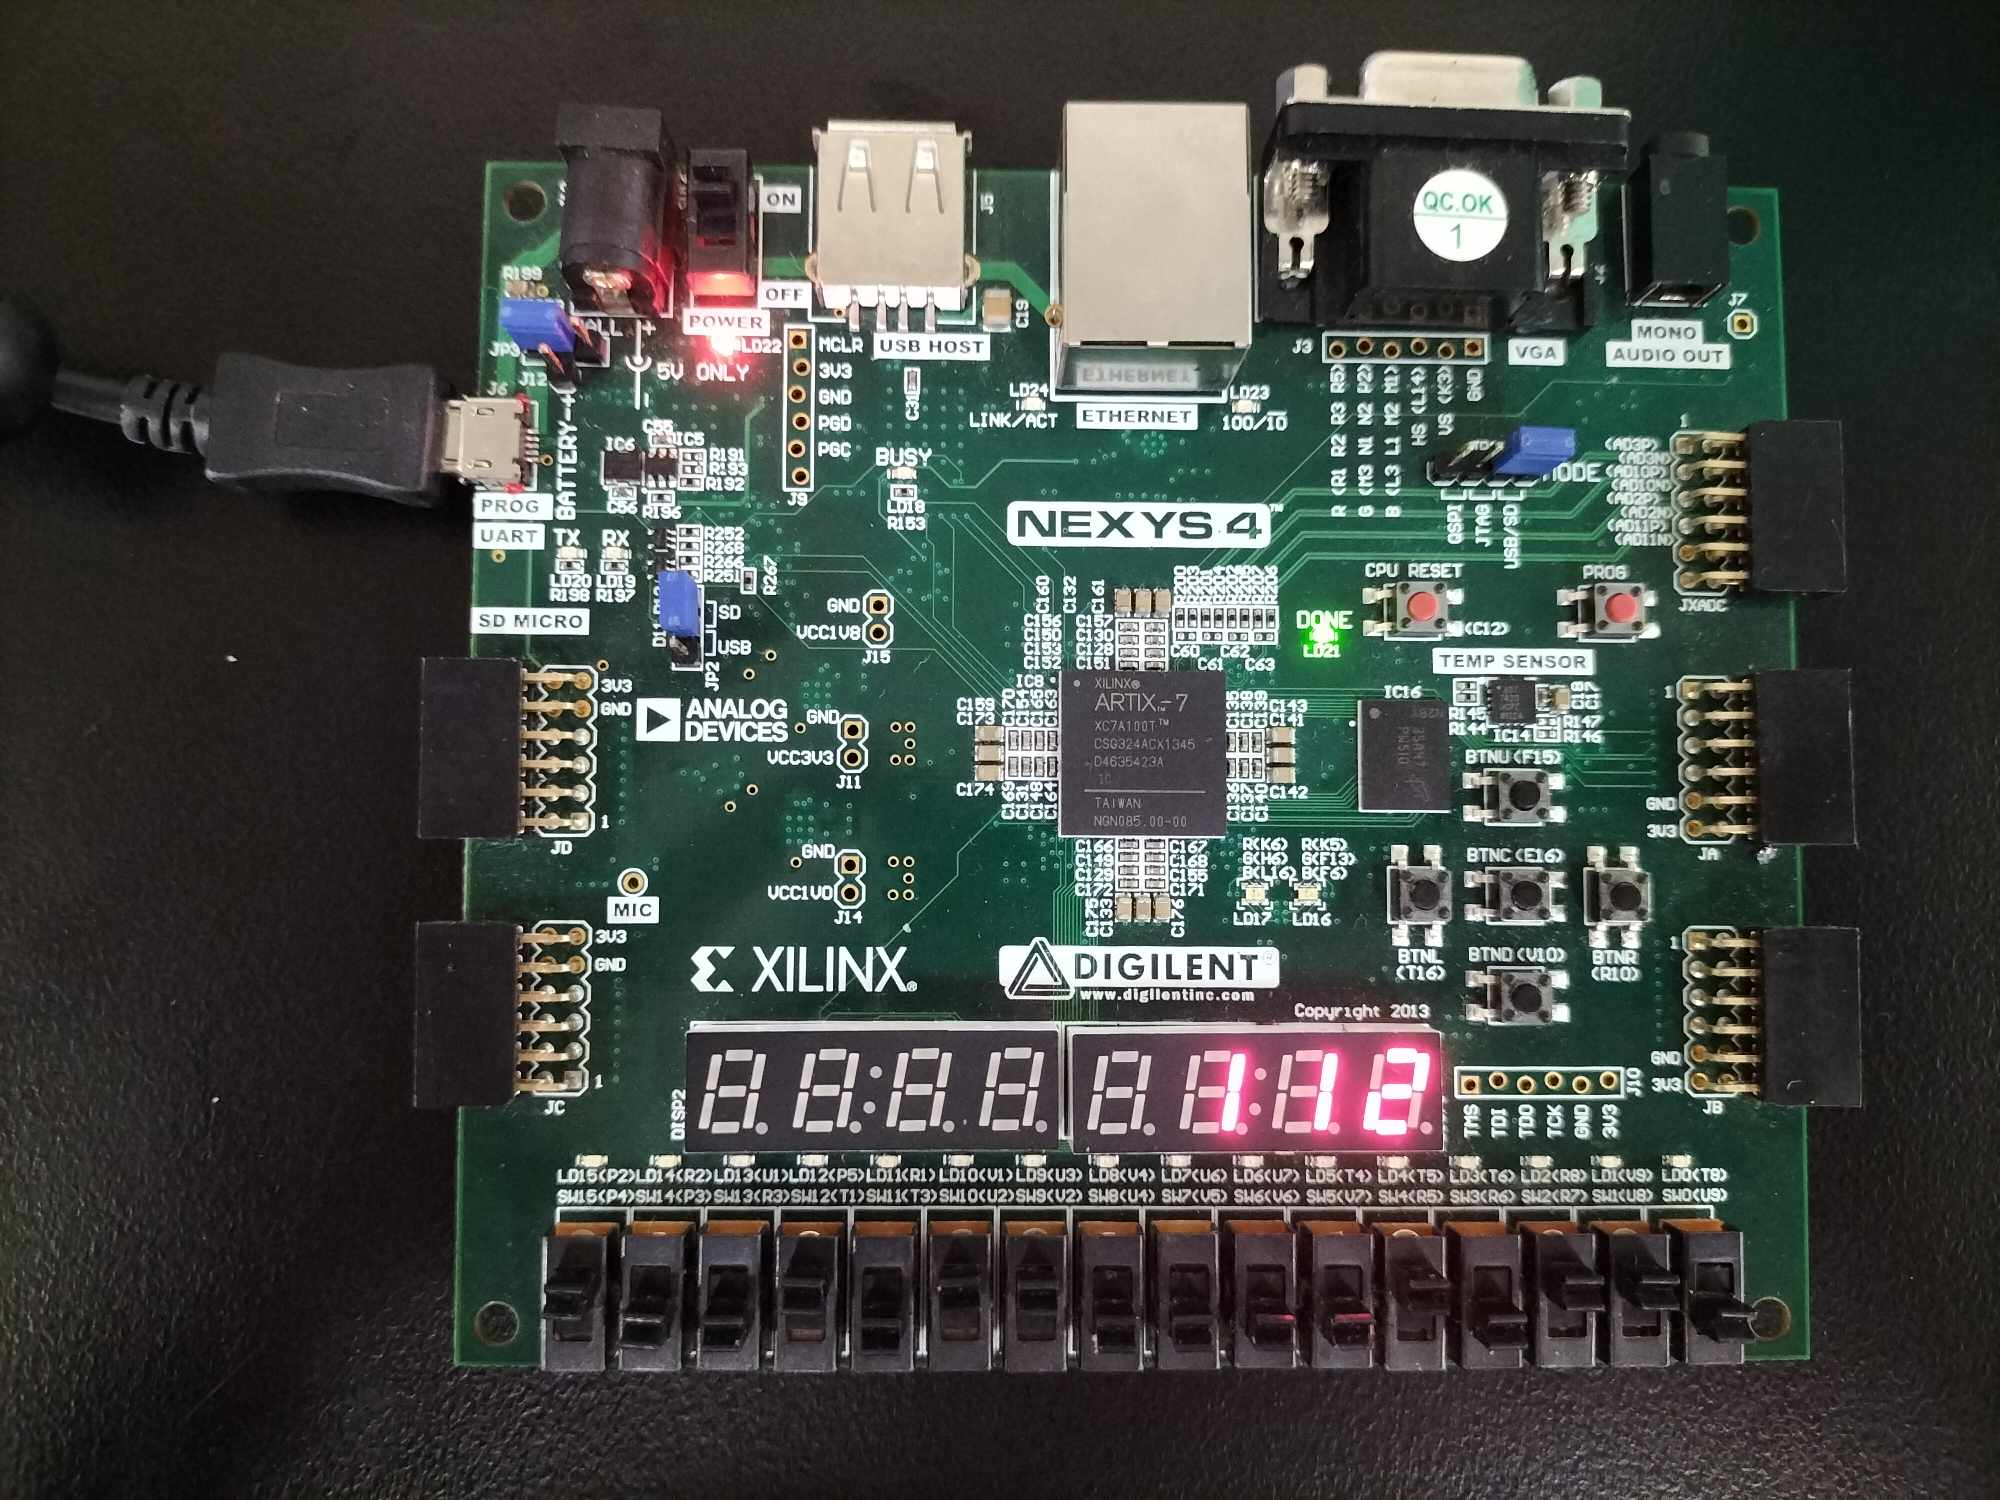
\includegraphics[scale=0.1]{images/fpga_two_overflow.jpg}
    \caption{FPGA with an overflow on both the higher and lower digits}
    \label{fig:fpga_two}
\end{figure}

\section{Register Transfer Level Schematic}

Figure \ref{fig:rtl} shows the top level design of the RTL schematic. This is going to be explained in greater detail in this segment.

\begin{figure}[H]
    \centering
    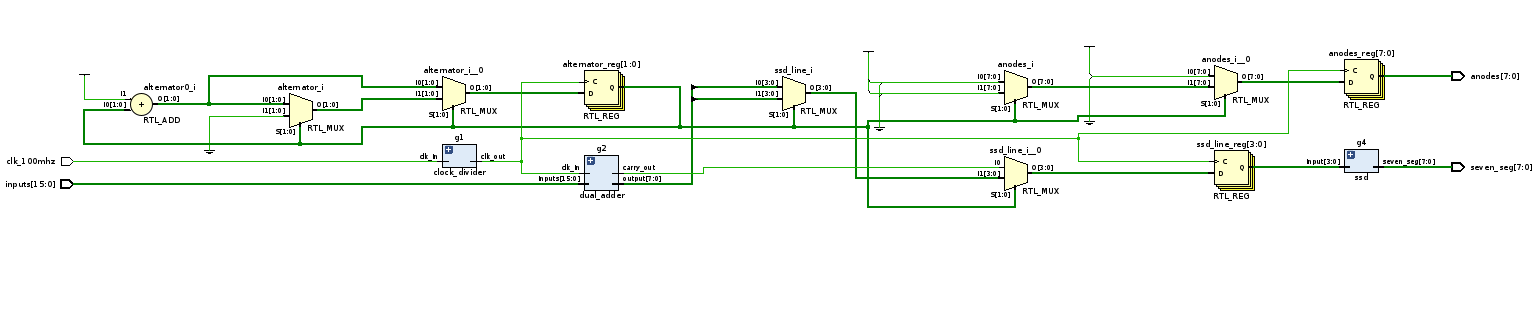
\includegraphics[scale=0.1]{images/rtl_whole.png}
    \caption{Register Transfer Level top level view}
    \label{fig:rtl}
\end{figure}

Figure \ref{fig:rtl} shows many similarities to the block diagram proposed at the beginning of this report. Asides from the finite state machine, which is represented with the alternator clock lines at the top of the RTL schematic, the rest of the diagram is near identical. The similarities become less apparent when taking a deep dive into the subsystems within the overall design. Figure \ref{fig:rtl_clk_div} shows the RTL schematic for the clock divider subsystem.

\begin{figure}[H]
    \centering
    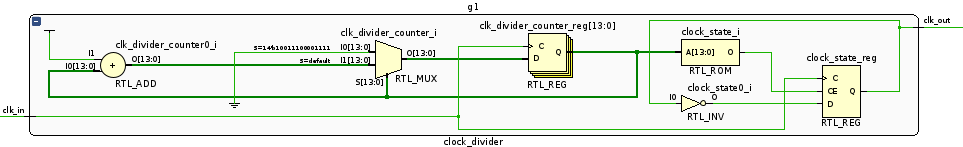
\includegraphics[scale=0.25]{images/rtl_clk_div.png}
    \caption{Register Transfer Level view of the clock divider subsystem}
    \label{fig:rtl_clk_div}
\end{figure}

The clock divider circuit shows a hardware implementation of the logic that was used to define it. The logic for the clock divider is as follows:

\begin{minted}{Python}
process (clk_in)
    begin
        if rising_edge(clk_in) then
            if (clk_divider_counter = n-1) then
                clk_divider_counter <= 0;
                clock_state <= not clock_state;
            else
                clk_divider_counter <= clk_divider_counter + 1;
            end if;
        end if;
    end process;

clk_out <= clock_state;
\end{minted}

As can be seen within this code logic, a counter is implemented, which is stored in a register which keeps on counting up. This is manifested within the left half of the RTL design, where the multiplexer is feeding into a register. The right hand side of the RTL design is concerned with the alternating of the clock state, which is manifested by a flip-flop connected to an inverter. This will flip the state of the clock every time the left-hand side has counted up to it's overflow value.

\begin{figure}[H]
    \centering
    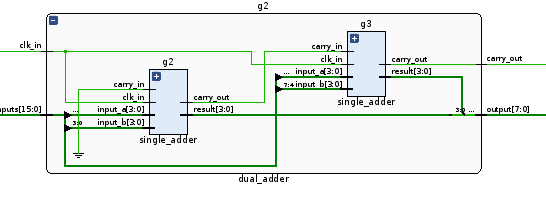
\includegraphics[scale=0.25]{images/rtl_dual_adder.png}
    \caption{Register Transfer Level view of both BCD adder subsystems}
    \label{fig:rtl_dual_adder}
\end{figure}

Figure \ref{fig:rtl_dual_adder} shows the schematic of the two BCD adders put together. As can be seen, the first adder receives a carry-in input of 0 from ground, while receiving input lines from the thick buffer. The carry out from the first adder is transferred to the second, which also receives two inputs from the thick buffer. In terms of inputs and outputs, this system is identical to the proposed block diagram.

\begin{figure}[H]
    \centering
    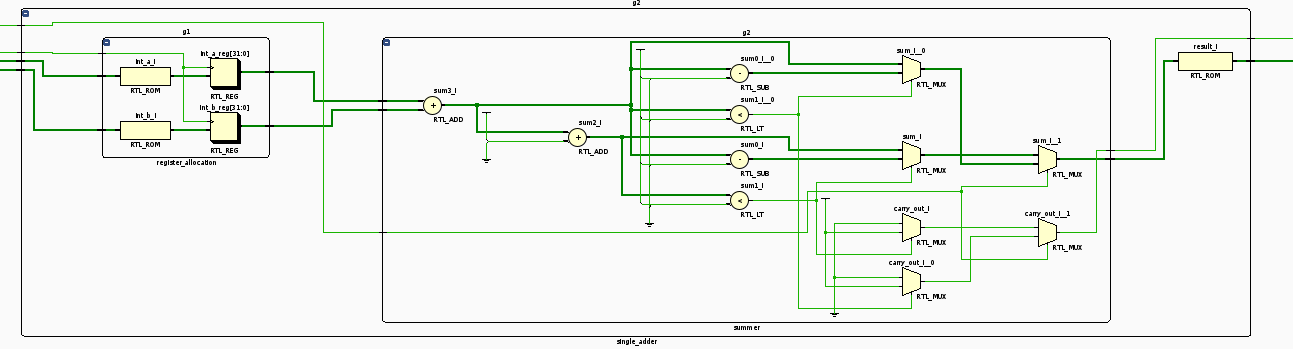
\includegraphics[scale=0.25]{images/rtl_single_adder.png}
    \caption{Register Transfer Level view of a single BCD adder}
    \label{fig:rtl_single_adder}
\end{figure}

Figure \ref{fig:rtl_single_adder} shows the RTL schematic of a single adder. Not really going to pretend to know what's going on with this one.

\begin{figure}[H]
    \centering
    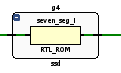
\includegraphics[scale=0.25]{images/rtl_ssd.png}
    \caption{Register Transfer Level view of the seven-seg decoder}
    \label{fig:rtl_ssd}
\end{figure}

Figure \ref{fig:rtl_ssd} is the final component of the RTL schematic. This component represents a seven-segment decoder that takes a 4-bit input and outputs the 8-bits required for the seven-seg display. In the RTL schematic it is represented simply by a single block.


\section{Synthesis Results}

There were several key features worth considering in the synthesis of the model. The most important of these is the memory usage of the design. Figure \ref{fig:memory} shows that less than $1\%$ of the entire system's memory was used in terms of look-up tables and registers. Furthermore, $16\%$ of the system's IO blocks were used in this design.

\begin{figure}[H]
    \centering
    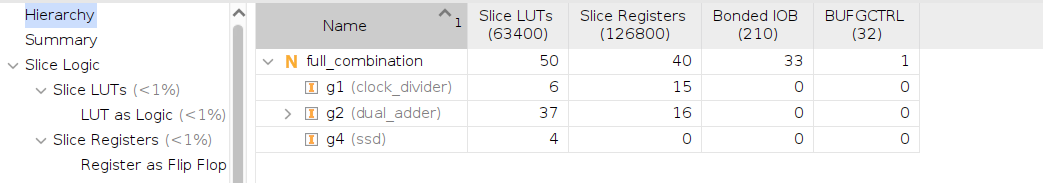
\includegraphics[scale=0.25]{images/synthesis_utilisation.png}
    \caption{Memory utilisation following synthesis}
    \label{fig:memory}
\end{figure}

The other important component of the model's synthesis was to ensure that synchronicity is attained, and that the design is able to function without timing errors. This is shown in figure \ref{fig:timing}, which shows that no slack exists in the design. It is worth mentioning that the previous practical featured a bug that introduced some degree of negative slack, as well as combinatorial logic loops that destabilised the clocking speed of the device. This error has since been addressed and is removed from practical 3.

\begin{figure}[H]
    \centering
    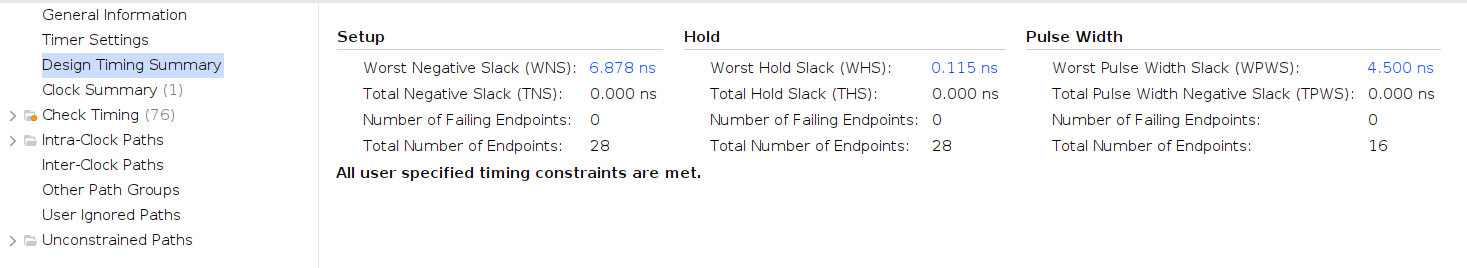
\includegraphics[scale=0.25]{images/synthesis_timing.png}
    \caption{Timing of the synthesis showing that there are no failings with timing during implementation}
    \label{fig:timing}
\end{figure}

\section{Conclusion}

In conclusion, both systems worked exactly as intended. The system for part 3A was able to create a 16-bit adders that provided all necessary functionality. Part 3B was a slightly more complex two-digit BCD adder, which was also created to satisfy the necessary design requirements. This time, there is no required places for improvement. It functions fully, while consuming less than 1$\%$ of the FPGA's resources. 

\end{document}
